\documentclass{article}
% \usepackage[margin=1in,footskip=0.25in]{geometry}
\usepackage{hyperref}
\usepackage{graphicx}
\usepackage[T1]{fontenc}
\usepackage{listings}
\usepackage{xcolor}
 
\definecolor{codegreen}{rgb}{0,0.6,0}
\definecolor{codegray}{rgb}{0.5,0.5,0.5}
\definecolor{codepurple}{rgb}{0.58,0,0.82}
\definecolor{backcolour}{rgb}{0.95,0.95,0.92}
 
\lstdefinestyle{mystyle}{
    backgroundcolor=\color{backcolour},   
    commentstyle=\color{codegreen},
    keywordstyle=\color{magenta},
    numberstyle=\tiny\color{codegray},
    stringstyle=\color{codepurple},
    basicstyle=\ttfamily\footnotesize,
    breakatwhitespace=false,         
    breaklines=true,                 
    captionpos=b,                    
    keepspaces=true,                 
    numbers=left,                    
    numbersep=5pt,                  
    showspaces=false,                
    showstringspaces=false,
    showtabs=false,                  
    tabsize=2
}
 
\lstset{style=mystyle}


\usepackage[margin=1in,footskip=0.25in]{geometry}
\usepackage{hyperref}
\usepackage{graphicx}
\usepackage[T1]{fontenc}
\usepackage{listings}
\usepackage{xcolor}
 
\definecolor{codegreen}{rgb}{0,0.6,0}
\definecolor{codegray}{rgb}{0.5,0.5,0.5}
\definecolor{codepurple}{rgb}{0.58,0,0.82}
\definecolor{backcolour}{rgb}{0.95,0.95,0.92}
 
\lstdefinestyle{mystyle}{
    backgroundcolor=\color{backcolour},   
    commentstyle=\color{codegreen},
    keywordstyle=\color{magenta},
    numberstyle=\tiny\color{codegray},
    stringstyle=\color{codepurple},
    basicstyle=\ttfamily\footnotesize,
    breakatwhitespace=false,         
    breaklines=true,                 
    captionpos=b,                    
    keepspaces=true,                 
    numbers=left,                    
    numbersep=5pt,                  
    showspaces=false,                
    showstringspaces=false,
    showtabs=false,                  
    tabsize=2
}
 
\lstset{style=mystyle}

\begin{document}

\title{
{\textbf{CS591S1 Homework 2: Main Report}\\
\large{Explore the Utility in Differentially Private Bayesian Inference}}
}
\author{Jiawen Liu\\
Collaborators: none.}

\date{}
\maketitle

\section{Abstract}
This project focus on protecting the data privacy in Bayesian analysis process, especially in a differentially private manner.
It starts from existing literatures, summarized popular differentially private Bayesian inference models and their main results in terms of utility under different problem settings.
Then this project studied the connections between these differentially private Bayesian inference models,
and their common utility properties. At the end, 


\paragraph{Keywords:} data analysis, Bayesian inference, differential privacy, utility optimization, utility trade-off.

\section{Introduction.}
Modern data analysis techniques have enabled significant
advances in a variety of applications in medicine, finance,
social science, and transportation. Privacy risk occurs when individual users contributes their data, in order to obtain better
services, these applications need large amounts of users’ data. 
Differential privacy was proposed a decade ago to address privacy concerns in these situations, and is now the standard for privacy-preserving data analysis.
While the privacy is always achieved at the expense of sacrificing utility, the trade-off between privacy and utility comes to the light.
Since most of the statistical applications are driven by Bayesian inference, this project will focus on the utility and privacy for differentially private Bayesian inferences, especially on inference tasks based on two classical statistical models: the Beta-Binomial model and Linear regression model.
This is a standard statistical tool in which a prior distribution is combined
with a sample of observed data in order to estimate a new posterior distribution.

The goal of this project is to explore the connections between differentially private Bayesian
inference mechanisms, in terms of utility and privacy, under different restrictions and different accuracy measurements (KL divergence, the Hellinger
distance, $l_k$ norm, etc.) over posterior distributions.
%
%

This project builds on some recent surprising works (\cite{ghosh2012universally}, \cite{zhang2016differential}, \cite{bernstein2020noise}) showing the optimality of differentially private Bayesian inference under specific restrictions. This line of work shows that when Bayesian inference is developed under a specific model in a certain differentially private way, the utility can achieve the optimality amount all kinds of privacy protection methods.
Thus the technique core of this project is to study the connections between these optimizations. 
Especially, there are many other works (\cite{bernstein2019differentially}) on differentially private Bayesian inference that haven't shown optimality.   
From the fundamental perspective, this project study their common utility properties.
%
\paragraph{Contributions.}
This project will systemically study existing differentially private Bayesian inference works in terms of their pre-assumptions/restrictions, structures, utilities and privacy.

\begin{itemize}
	\item Summary of existing structures of differentially private Bayesian inference works under different specifications.
%
	\item New study of the connections between utility optimality of different differentially private Bayesian inference structures. 
%	
	\item New study on the fundamental of the utility over all differential kind of the differentially private Bayesian inference.
%
\end{itemize}

\section{Preliminaries}
\paragraph{Bayesian Inference}
\noindent \textbf{Bayesian inference.} 
Given a prior belief $\Pr(\theta)$ on some parameter $\theta$,
and an observation $\dataobs$, the posterior distribution on $\theta$
given $\dataobs$ is defined by Bayes' Theorem as:
\[
  \Pr(\theta | \dataobs) = \frac{\Pr(\dataobs | \theta) \cdot \Pr(\theta)}{\Pr(\dataobs)}
\]
where the expression $\Pr(\dataobs | \theta)$ denotes the
\emph{likelihood} of observing $\dataobs$ under a value of
$\theta$. 
% Since we consider $\dataobs$ to be fixed, the likelihood is
% a function of $\theta$.
% For the same reason $\Pr(\dataobs)$ is a constant independent of $\theta$.
% Usually in statistics the prior distribution $\Pr(\theta)$ is chosen so that it represents
% the initial belief on $\theta$, that is, when no data has been
% observed. In practice though,
In parametric statistics, prior distributions and likelihood functions are usually chosen so that the posterior
belongs to the same \emph{family} of distributions as the prior. In this case we say that the prior
is conjugate to the likelihood function. Use of a conjugate prior
simplifies calculations and allows for inference to be performed in a
recursive fashion over the data. This approach is implemented in a
precise or approximate way in the compiler of several
probabilistic programming languages~\cite{BartheFGAGHS16}.
%
%
\paragraph{Exponential Family}
The Bayesian Inference in an exponential family is considered in this project. Given the same setting as above, the exponential family in natural parameterization has density:
%
\[
	\Pr(x | \theta) = h(x) \exp(\theta^{T} t(x) - A(\theta)),
\]
%
where $\theta$ are the natural parameters, $t(x)$ is the sufficient statistic,
$A(\theta) = \int h(x) \exp(\theta^T t(x))$
is the log-partition function, and $h(x)$ is the base measure.
The density of the full data is
\[
	\Pr(\dataobs | \theta) = 
	h(\dataobs) \exp(\theta^{T} t(\dataobs) - nA(\theta)),
\]
%
where $h(\dataobs) = \prod h(\dataobs_i)$ and 
$t(\dataobs) = \sum t(\dataobs_i)$.
%
Every exponential family distribution havs a conjugate prior distribution $p(\theta; \lambda)$
with hyperparameters $\lambda$. 
A conjugate prior has the property that, if it is used as the prior, 
then the posterior belongs to the same family, i.e., $\Pr(\theta | \dataobs; \lambda) = p(\theta;\lambda')$ 
for some $\lambda'$ that depends only on $\lambda, n$ and the sufficient statistics $s$.
%
Our following research will focus on some specific models in this exponential family. 

\paragraph{Differential Privacy}
%
%
\emph{Differential privacy}~\cite{dwork2006} is a quantitative notion
of data privacy guaranteeing  a bound on the that changing the input of a mechanism slightly only reflects
in a controlled and bounded way on the output distribution. 
Formally, the $\epsilon$ parameter
controls how much two outputs starting from \emph{close} inputs can differ. When two inputs are close we call them \emph{adjacent}.
By adjacency we usually mean a relation over input databases which includes all the pair of databases which differ by at most one row.
The formal definition of $\epsilon$-differential privacy follows.
\begin{definition}
\label{def_epsilon_dp}

A randomized mechanism $\mathcal{M}$ with domain $\mathbb{N}^{|\mathcal{X}|}$ and codomain $\range$, is $\epsilon$-differential private, if for all adjacent
\footnote{Given $\dataobs, \dataobs'\in\{0,1\}^n$  we say that $\dataobs$ and $\dataobs'$ are adjacent and we write, iff
$\sum_{i}^{n}\iverson{x_i = x'_i }\leq 1$. } $\dataobs, \dataobs' \in \mathbb{N}^{|\mathcal{X}|}$ and all $\mathcal{S} \subseteq \range$:
\begin{equation*}
\Pr[\mathcal{M}(\dataobs) \in \mathcal{S}] \leq e^\epsilon \Pr[\mathcal{M}(\dataobs') \in \mathcal{S}].
\end{equation*}

\end{definition}


It is possible to achieve $\epsilon$-differential privacy through use and composition of
a few basic components. Some of these components are now reviewed.
%
%
\section{Differentially Private Bayesian Inference Models}
%
This section introduced three kind of differentially private Bayesian inference Models we will study in detail in following works as shown in Figure \ref{fig_pinfermodel}. 
\begin{figure*}[t!]
    \centering
    \begin{subfigure}[t]{0.3\textwidth}
        \centering
        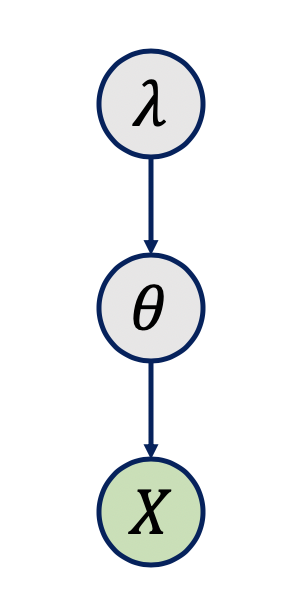
\includegraphics[height=1.2in]{nonp.png}
        \caption{Non Private Bayesian Inference}
    \end{subfigure}%
    ~ 
    \begin{subfigure}[t]{0.3\textwidth}
        \centering
        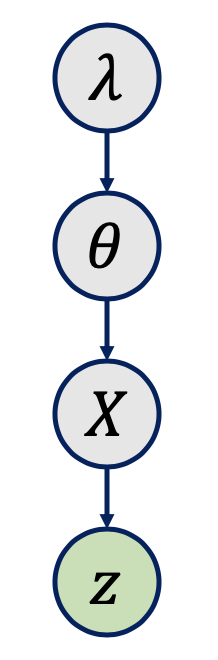
\includegraphics[height=1.2in]{pinfer}
        \caption{Private Bayesian Inference on Data}
    \end{subfigure}
    ~ 
    \begin{subfigure}[t]{0.3\textwidth}
        \centering
        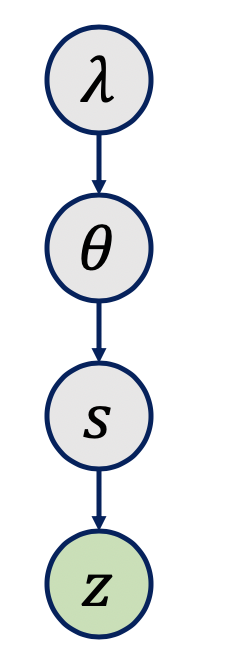
\includegraphics[height=1.2in]{pinferons}
        \caption{Private Bayesian Inference on Sufficient Statistics}
    \end{subfigure}
    \caption{Private Bayesian Inference Model}
    \label{fig_pinfermodel}
\end{figure*}
\subsection{Non-private Inference}
%
As shown in Figure \ref{fig_pinfermodel}(a), the non-private inference graph start from the hyper parameter following the Bayesian inference process in exponential family.
%
Then it will directly release the full data without any manipulation on data.

\subsection{Private Inference over Data}
%
As shown in Figure \ref{fig_pinfermodel}(b), 
the private inference over data start with the same pre-procedure as non-private model with the same hyper-parameter and prior distribution.
%
Then instead of release the data directly, it perform the analysis and release a perturbed quantity $z$.
%
In this way, the noise model due to the release mechanism can be directly accounted for in a probabilistic inference procedure, 
with the intent of producing more principled and higher-utility private analyses.
%
\\
The key insight is that exposing the details of the release mechanism does not harm the differential privacy guarantee. 
Given release mechanisms are made public,
the knowledge of the mechanism defines the conditional distribution $\Pr(z |\dataobs)$,
which can be combined with the generative data model, $\Pr(\dataobs | \theta)$, to form a new likelihood distribution on data:
\[
\Pr(z | \theta) = 
\int
\Pr(\dataobs | \theta)
\Pr(z |\dataobs) d \dataobs.
\] 
%
Thus the main technique developed under this model is to form approximations of this integral and obtain either a closed form or a tractable sampling procedure.

\subsection{Private Inference over Sufficient Statistics}
%
As shown in Figure \ref{fig_pinfermodel}(c), instead of working with individual data directly,
this model works with the sufficient statistics,
where the sufficient statistics are quantities
that capture all information about the model parameters (\cite{foulds2016theory}, \cite{vu2009differential}).
%
In this model, noises are added to these sufficient statistics and then Bayesian inference analysis are performed on these noisy statistics where the analysis results will finally be released. 
%
\\
%
This project will study some specific problems and algorithms mainly under this model and then focus on the connections and difference between the two models.
%
\section{Private Bayesian Inference under Different Problem Settings}
%

\subsection{For Counting Query \texorpdfstring{\cite{ghosh2012universally}}{}}
%

\subsubsection{Problem Setting}
%
Following the model in Figure \ref{fig_pinfermodel}(c), this section studied under the setting:
\begin{itemize}
\item Data base be a set of bits.
\item the sufficient statistics are the result of counting queries with integer type.
\item The noise added to the statistics are integers from geometric distribution.
\end{itemize}
%
Below are some formal definitions which will be used in this model.
%
\begin{definition}[Counting Query]
\end{definition}

\begin{definition}[Geometric Mechanism]
\end{definition}

\begin{definition}[Utility Model]
\end{definition}

\subsubsection{Equivalence Between Private Inference and Geometric Noise}
%
For every rational user u,
the private inference process can be factored into a user-independent part
(the $\alpha$-geometric mechanism) followed by a user-dependent post-processing step.

\subsubsection{Main Theorem}
%
\begin{thm}
for each fixed count query and differential privacy level,
there is a geometric mechanism 
$M$ that is simultaneously expected loss-minimizing for every possible user,
subject to the differential privacy constraint.
\end{thm}

\subsection{For Linear Regression
\texorpdfstring{\cite{bernstein2019differentially}}{}}
%

\subsubsection{Problem Setting}
%
Again following the model in Figure \ref{fig_pinfermodel}(c), another popular problem studied under this model is Bayesian linear regression. 
%
Below are some formal definitions which will be used in this model.

%
\begin{definition}[Linear Regression]
\end{definition}

\begin{definition}[Private Linear Regression Model]
 sufficient-statistic perturbation
\end{definition}

\begin{definition}[Calibration Measures]
\end{definition}

\begin{definition}[Utility Measures]
\end{definition}
%
%
\subsubsection{Main Result}
%
The results are shown in experiments.

\subsection{For Posterior Inference
\texorpdfstring{\cite{Zhang2017privbayes}}{}}
%

\subsubsection{Problem Setting}
%
The same counting query as before.
\begin{definition}[Laplace Mechanism]
\end{definition}

\begin{definition}[Probabilistic Graphical Models]
\end{definition}
\subsubsection{Main Theorem}
\begin{thm}[Utility Bounds on Posterior]
\end{thm}
%
%
\section{Connections Between Different Models}

\section{Experimental Results}

\section{Conclusion}
The summary of existing structures of DP-Bayesian inference works can help to develop some fundamental frameworks in this line. Then, the study of the connections between different utility optimality, and their common utility properties can help to develop new optimality for some other differentially private Bayesian work that haven't achieve optimality. This project will even build the framework for the differentially private Bayesian inference.


\newpage
\bibliographystyle{plain}
\bibliography{main.bib}



\end{document}
